\section{VGGNet}
2014'de ImageNet ILSVRC (Büyük Ölçekli Görsel Tanıma Yarışması)'de sunuldu. Yarışmayı, GoogleLeNet modelinden sonra tamamlayarak ikinci oldu. VGG Group (Oxford) tarafından sunulmuştur. Ağın derinliğinin önemi üzerinde durulmuştur. Farklı sürümleri de bulunur. AlexNet mimarisinde kullanılan yüksek kernel boyutları azaltılmıştır. Sadece 3x3 filtre ve 2x2 lik havuz boyutları kullanılarak ağa basit kazandırılmış ve derinlik korunmuştur.

\begin{figure}[h]
    \centering
    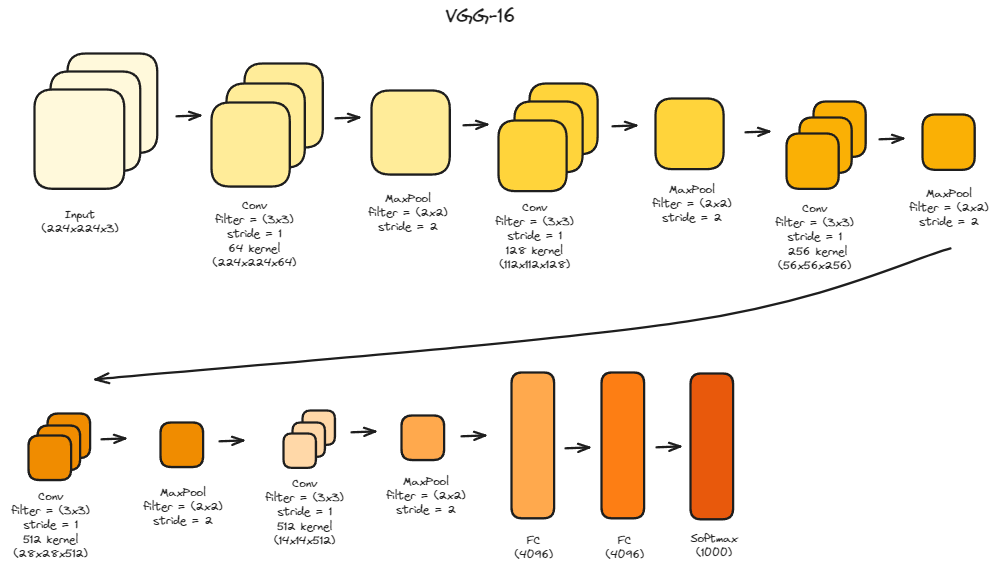
\includegraphics[width=1\textwidth]{images/vgg16.png}
    \caption{VGG16 mimarisi.}
    \label{fig:enter-label}
\end{figure}

\begin{lstlisting}[language=Python]
# VGG-16
model = Sequential([
	Conv2D(filters=64, kernel_size=(3,3), padding="same", activation="relu"),
	Conv2D(filters=64, kernel_size=(3,3), padding="same", activation="relu"),
	MaxPooling2D((2, 2)),
	
	Conv2D(filters=128, kernel_size=(3,3), padding="same", activation="relu"),
	Conv2D(filters=128, kernel_size=(3,3), padding="same", activation="relu"),
	MaxPooling2D((2, 2)),
	
	Conv2D(filters=256, kernel_size=(3,3), padding="same", activation="relu"),
	Conv2D(filters=256, kernel_size=(3,3), padding="same", activation="relu"),
	Conv2D(filters=256, kernel_size=(3,3), padding="same", activation="relu"),
	MaxPooling2D((2, 2)),
	
	Conv2D(filters=512, kernel_size=(3,3), padding="same", activation="relu"),
	Conv2D(filters=512, kernel_size=(3,3), padding="same", activation="relu"),
	Conv2D(filters=512, kernel_size=(3,3), padding="same", activation="relu"),
	MaxPooling2D((2, 2)),
	
	Conv2D(filters=512, kernel_size=(3,3), padding="same", activation="relu"),
	Conv2D(filters=512, kernel_size=(3,3), padding="same", activation="relu"),
	Conv2D(filters=512, kernel_size=(3,3), padding="same", activation="relu"),
	MaxPooling2D((2, 2)),
	
	Flatten(),
	Dense(4096, activation="relu"),
	Dense(4096, activation="relu"),
	Dense(1000, activation="softmax")					
])
\end{lstlisting}

\newpage